\section{Crops combination}
Since the neural network has been constucted in a way that the input size is 256 by 256 pixels, one cannot feed a bigger image in there. Therefore a high-resolution image has to first split into several crops which are then get recombined. There are several ways of how one can split the image, the easiest approach would be to use a sliding window. With the step size of $s$ and the window size of $w$ the sliding window is defined as: 

When step size $s$ is equal to window size $w$, there is no overlap between the windows. One very important insight from prediction results if that the model is less accurate on the borders of the image, rather than of cropping itself. Images are cropped consequently and most the times there are cells on the borders of the crops that get sliced and it might be impossible the make a good prediction for them just due to the lack of the information. Therefore the step size has to be smaller than the window size, so that the windows are overlapping and for each prediction we use only the image center and are allowed to ingore predictions on the border. 

Such approach would help to reduce the effect of the grid visible on the image composed of many small crops, which one can see in the Figure \ref{fig:crops_combination_0} to almost non-visible borders as in the Figure \ref{fig:crops_combination_34}. This would of course take longer time in predictions, however as the speed is less crucial in comparison to the accuracy of the predictions.

\begin{figure}[htb]
    \centering
    \begin{minipage}{.48\textwidth}
      \centering
      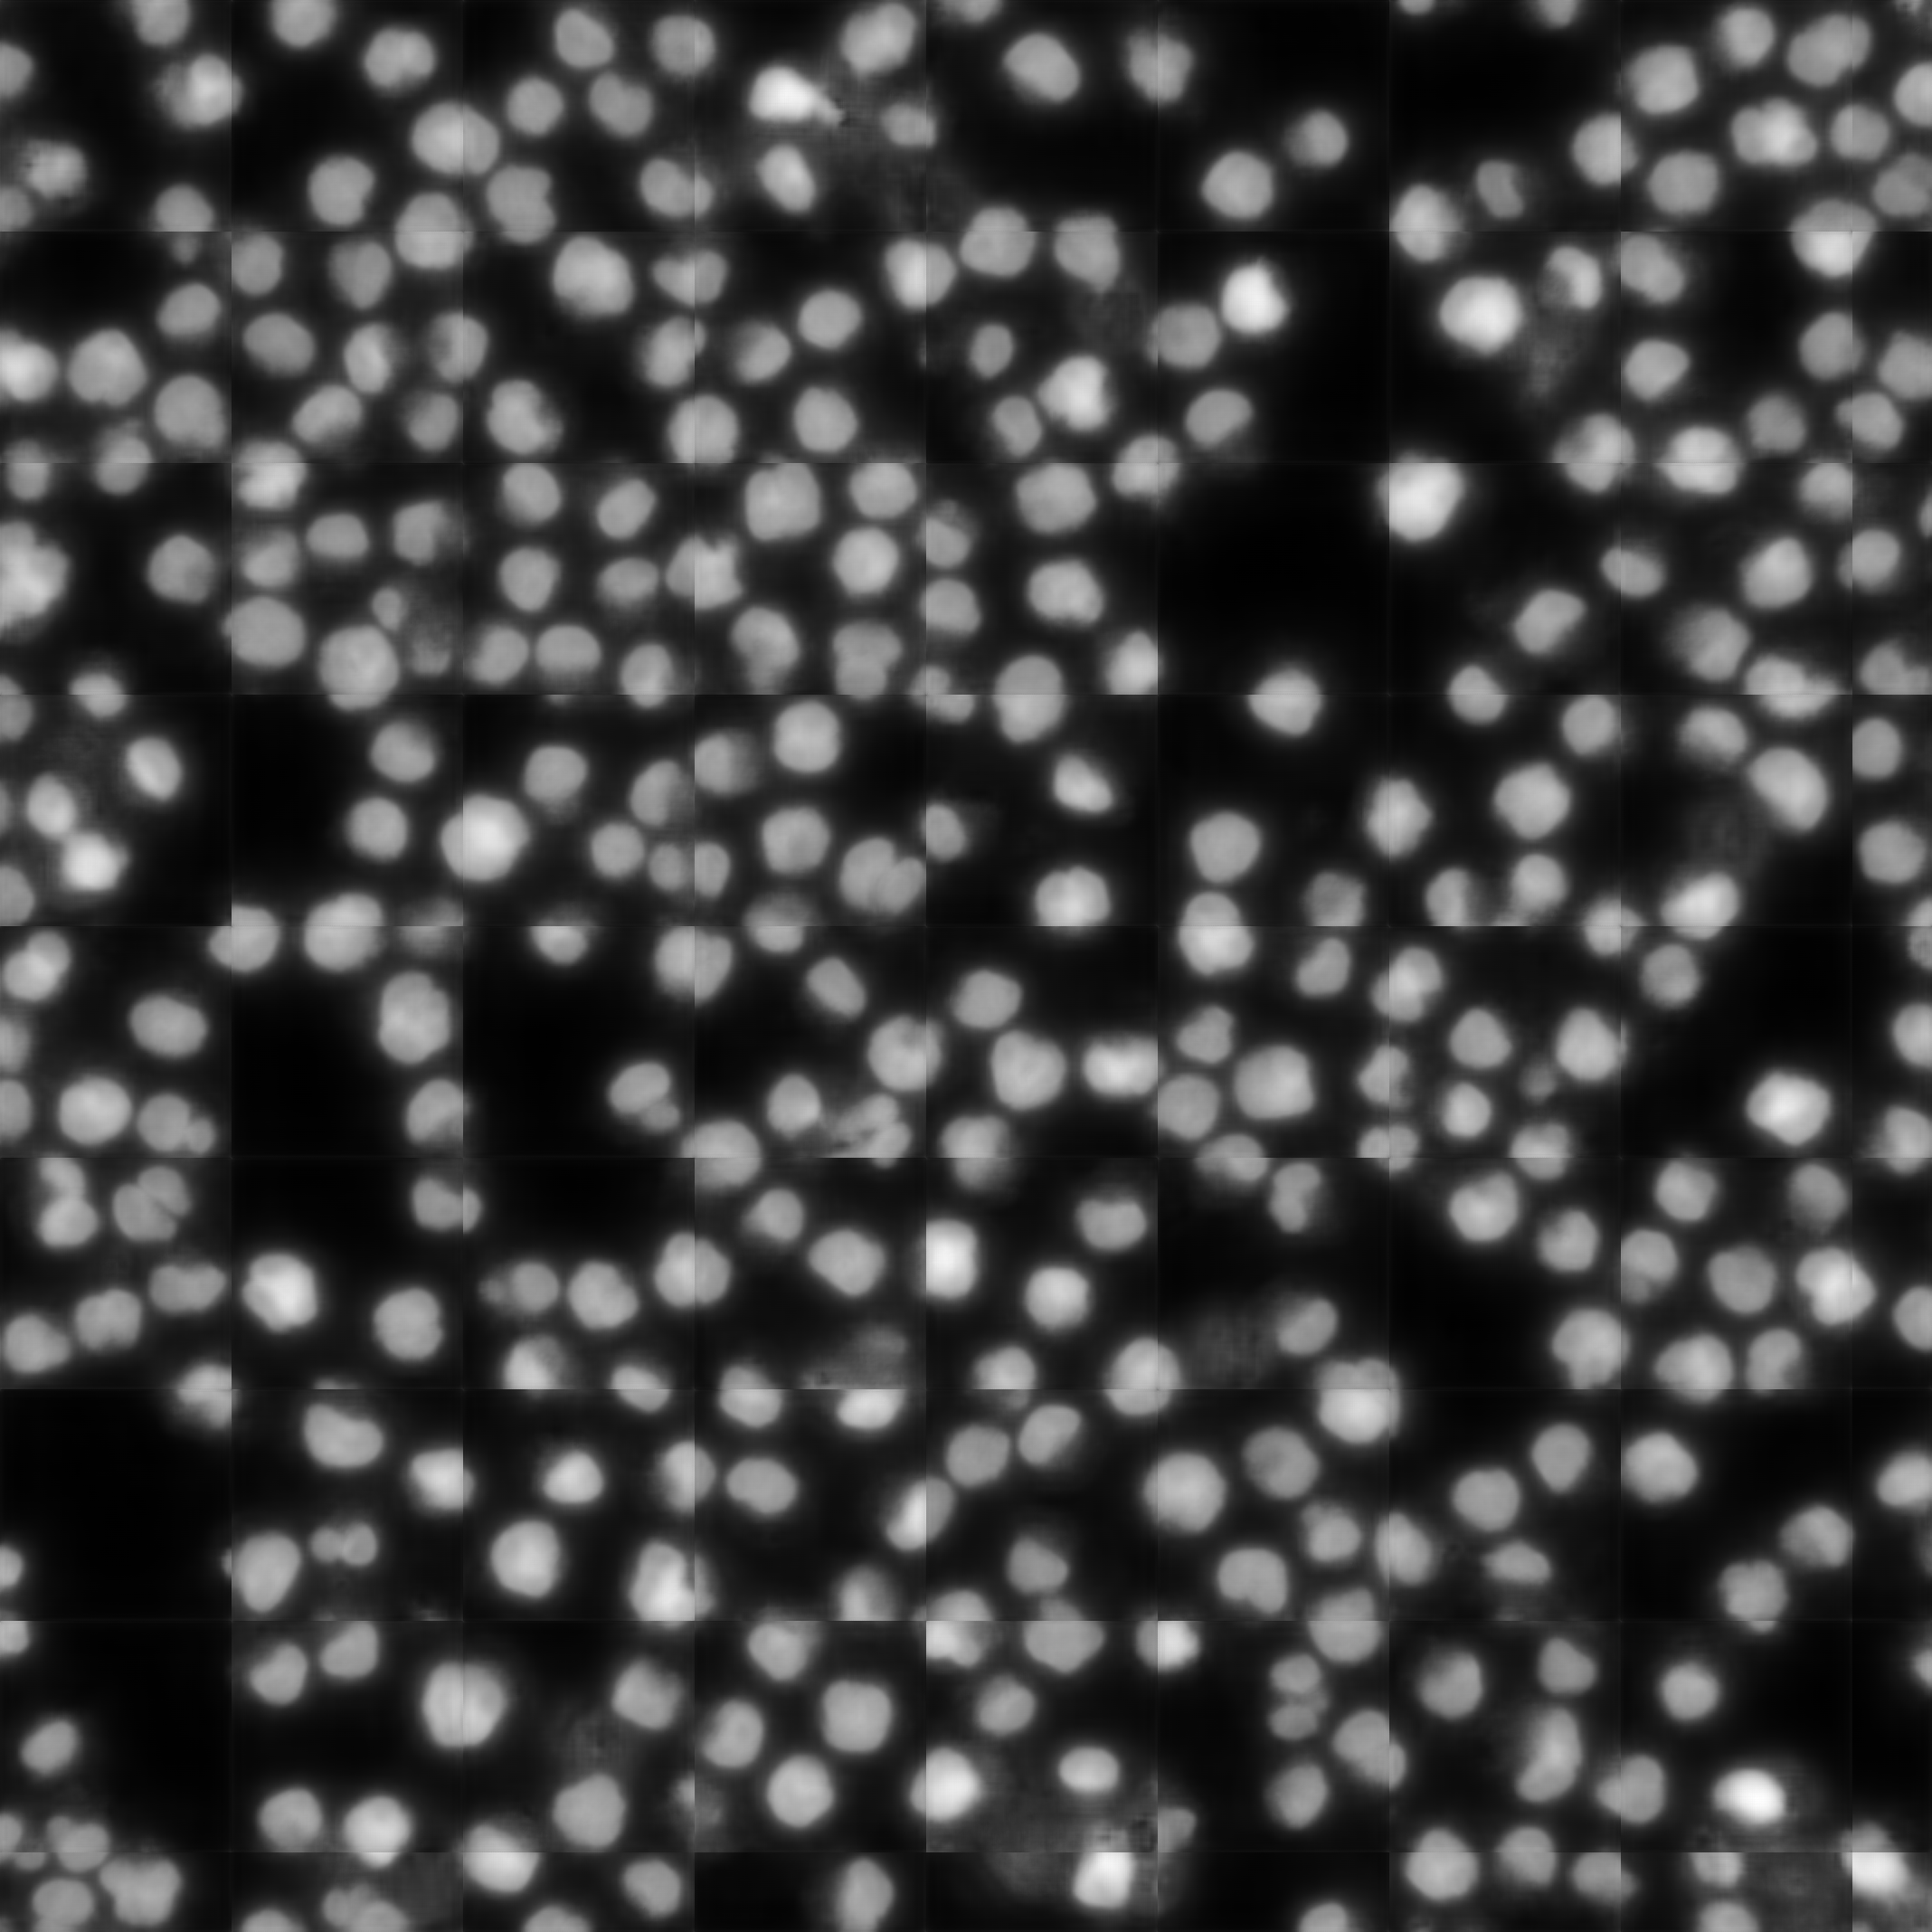
\includegraphics[width=\linewidth]{bilder/crops_combination/prediction_border_0.png}
      \caption{No overlap}
      \label{fig:crops_combination_0}
    \end{minipage}%
    \vspace{1cm}
    \begin{minipage}{.48\textwidth}
      \centering
      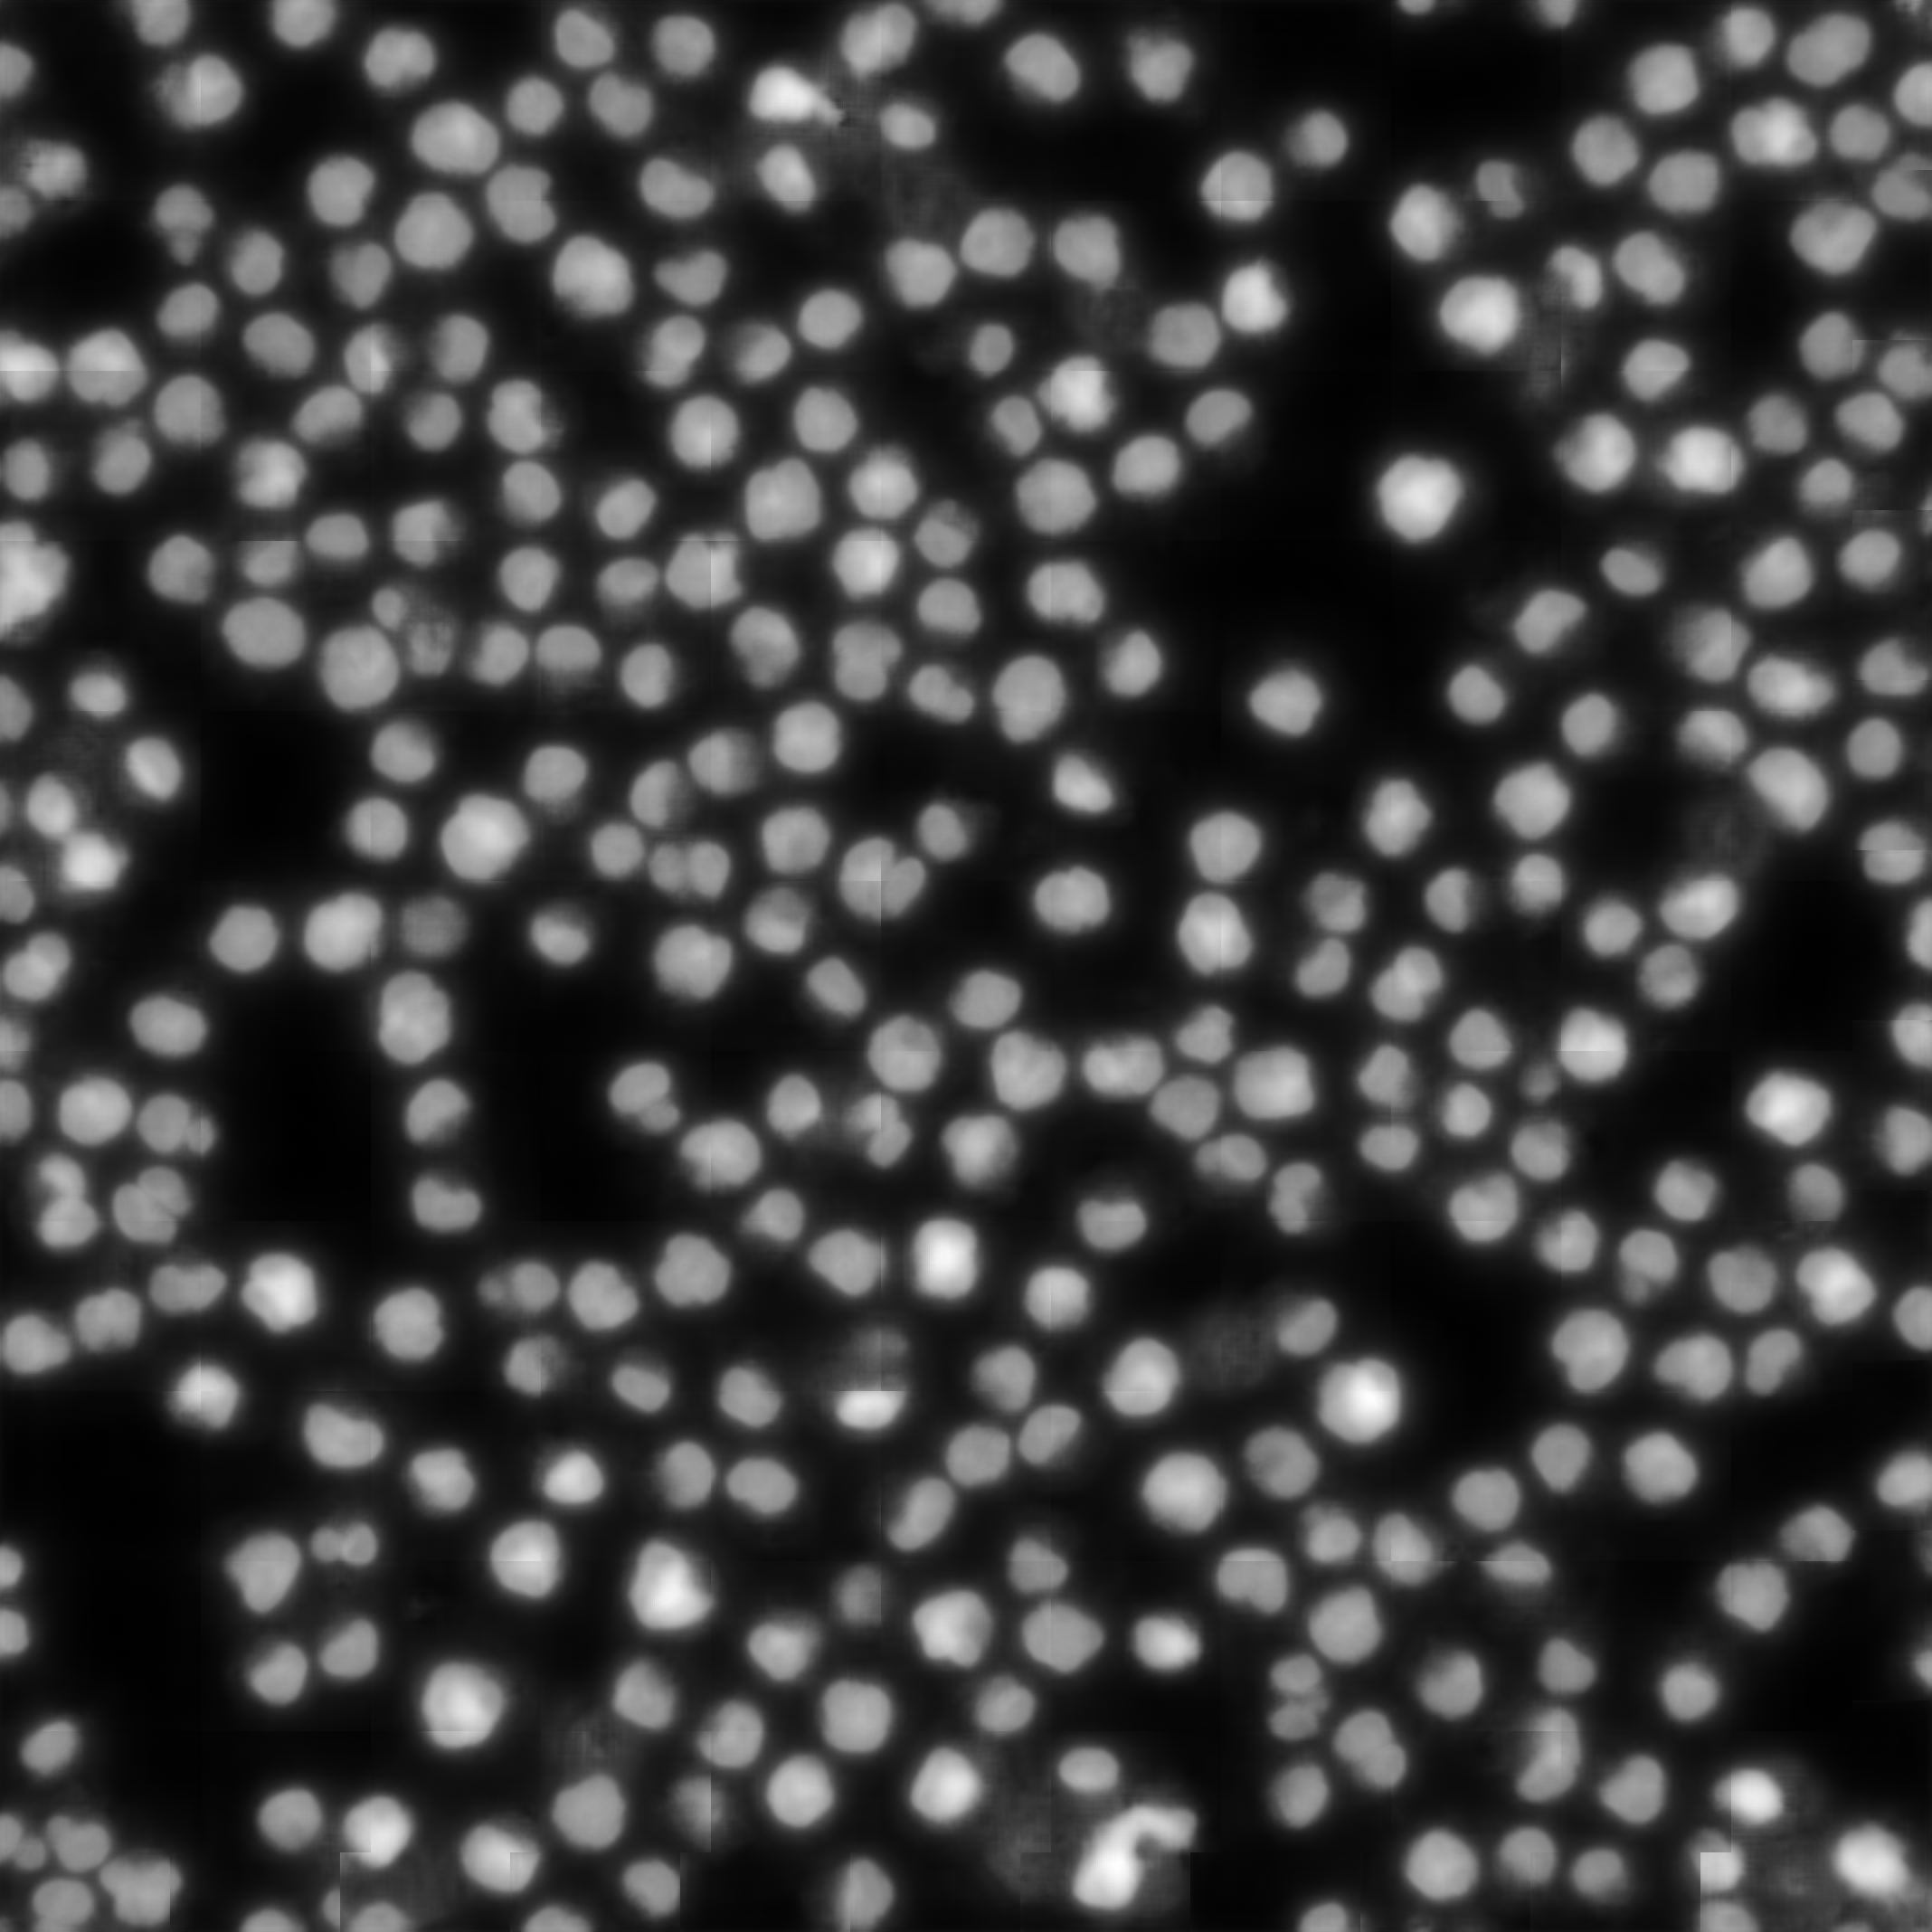
\includegraphics[width=\linewidth]{bilder/crops_combination/prediction_border_34.png}
      \caption{30 pixels overlap}
      \label{fig:crops_combination_34}
    \end{minipage}
\end{figure}